\section{Allocation}

As the allocator for the data structure, a bump allocator is used (also known as stack allocator). The bump allocator allocates a continuous linear section of memory and works by increasing a pointer at the next unused memory.

\begin{figure}
  \centering
  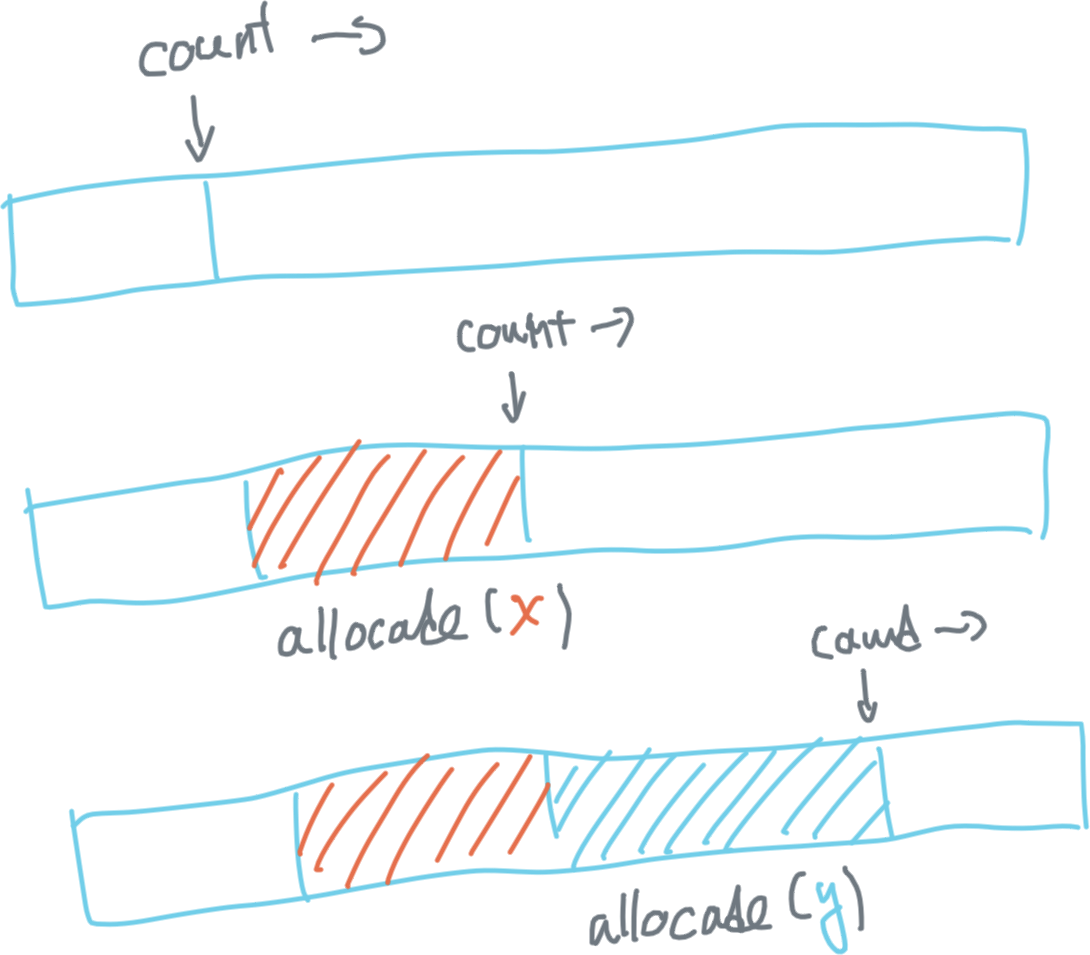
\includegraphics[width=0.8\textwidth ]{components/figure/bump-allocator}
  \caption{States of the tree during splitting while inserting a new key.}
  \label{figure:bump-allocator}
\end{figure}

To handle the allocation of nodes, a section of memory must be allocated beforehand on the CPU, as the device code cannot allocate additional memory by itself. A bump allocator is used in both of the TNL implementations.

Keeping track of the used size and the pointer to a next node with utilizing \code{atomicCAS}. Atomic instructions are used to ensure the serializability of the operations, as the allocator is invoked concurrently from different threads.

The main benefit is the simplicity of the allocator; the disadvantage is the lack of granular deallocation; it can only free all memory at once.
